To make it easier to read component diagrams, it was decided to present 4 diagrams. The first represents a high-level view that reports client-side and server-side components. The other 3 diagrams each represent one of the 3 main subsystems presented in the first diagram.
\subsection{High level component diagram}
    The following diagram shows the main components of the system and the interfaces through which they interact. There are 2 sides:
    \begin{itemize}
        \item The \textbf{client-side} is composed of 2 components: Mobile Application for the customers and Web Application for employees and the store manager
        \item The \textbf{server-side} is the significant part to analyze more thoroughly, here are 3 main subsystems: \begin{itemize}
            \item The \textit{Customer Mobile Services} provides the interfaces to line up, book a visit and manage historical information and account information
            \item The \textit{Employee Web Services} supports the operations that the employee can perform on the web application. This component provides the interfaces to line up (for an external client), to confirm an entrance or an exit from the store
            \item The \textit{Store Manager Web Services} supports the operations that the store manager can perform on the web application. This component provides the interfaces to manage store and employees information and to visualizes data about entrances
        \end{itemize}
    \end{itemize}

    \begin{figure}[H]
        \centering
        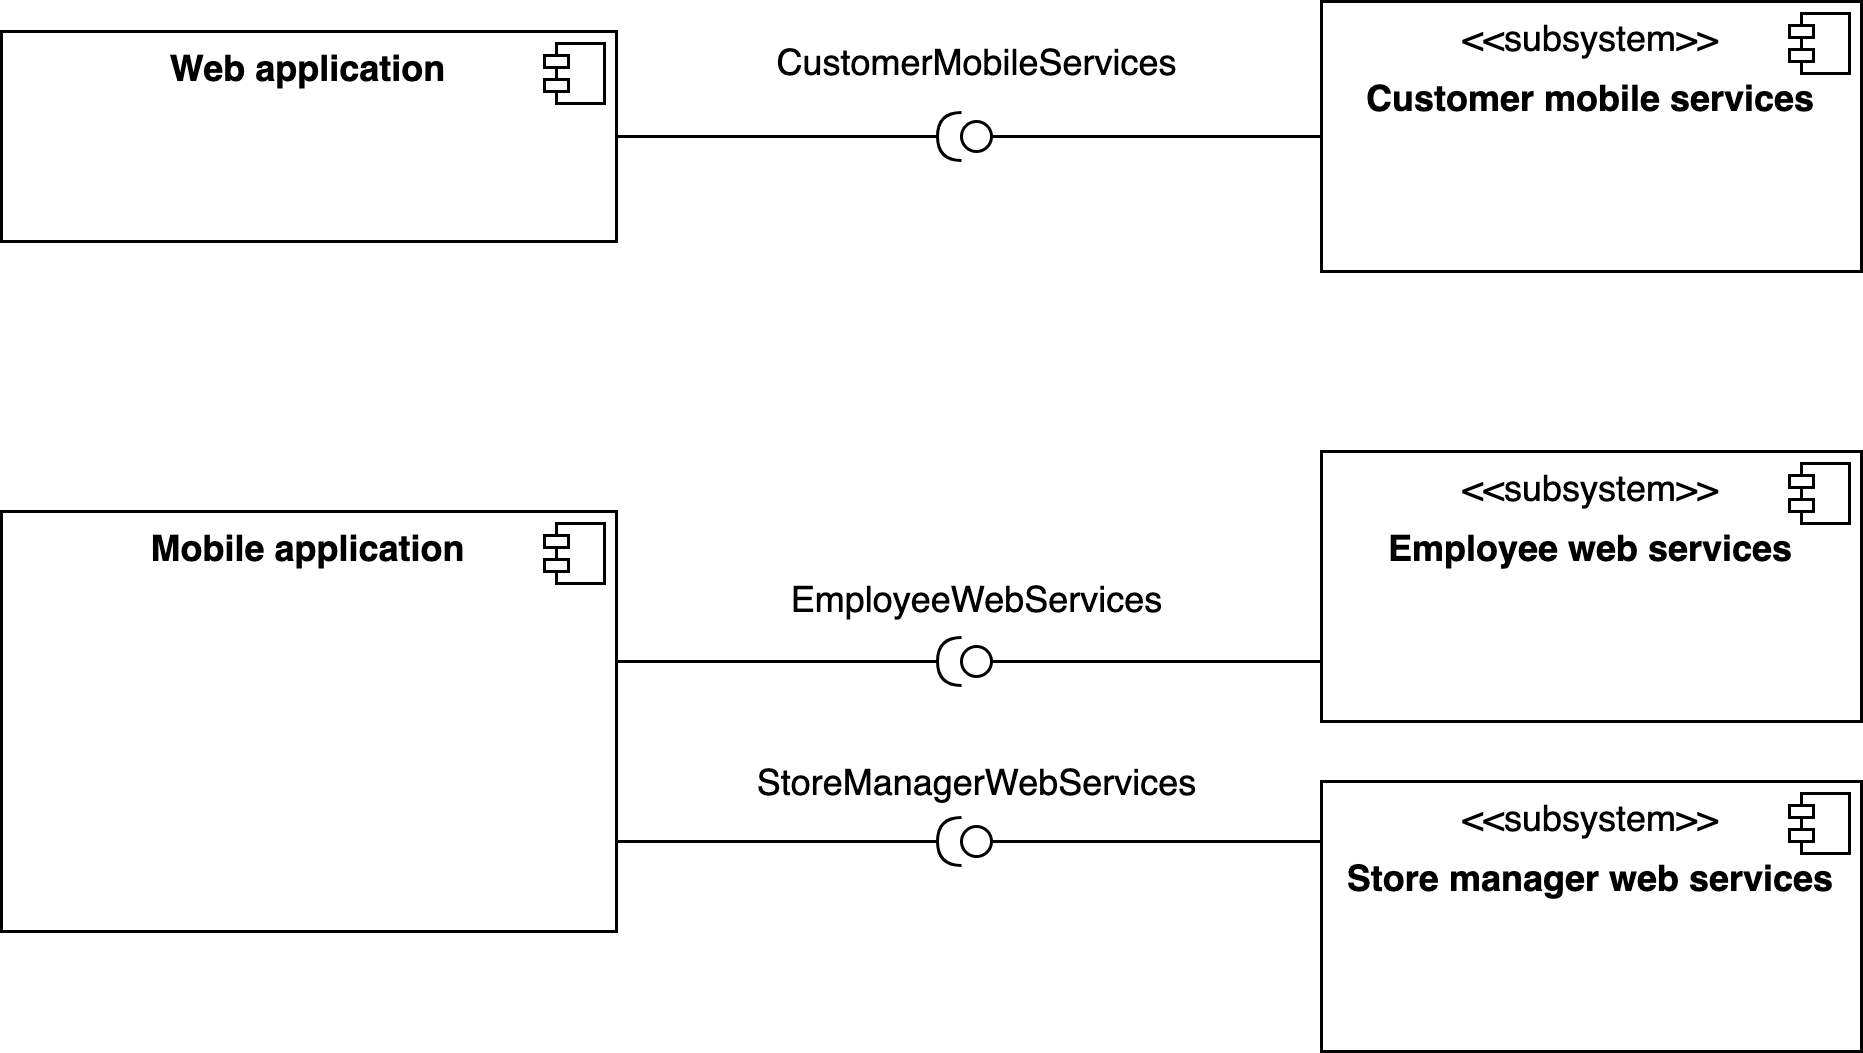
\includegraphics[width=16cm]{component_view-High-level.png}
        \caption{High level component diagram}
    \end{figure}

\subsection{Customer mobile services diagram}

    The following diagram shows how the subsystem \textbf{Customer Mobile Services} is composed and how its modules communicate with external modules. This subsystem contains 3 modules: a \textit{Visit Reservation Module}, a \textit{Line up Reservation Module} and an \textit{Account Manager}. This modules provides to Mobile Application the following interfaces: \textit{VisitHistory}, \textit{LineUpHistory}, \textit{ManageVisit}, \textit{ManageLineUp}, \textit{ProfileManagement}, \textit{AccessManager}. The components of the Customer Mobile Services subsystem need to communicate with the DBMS, Queue Manager and Visit Scheduler and indirectly with Maps API.

    \begin{figure}[H]
        \centering
        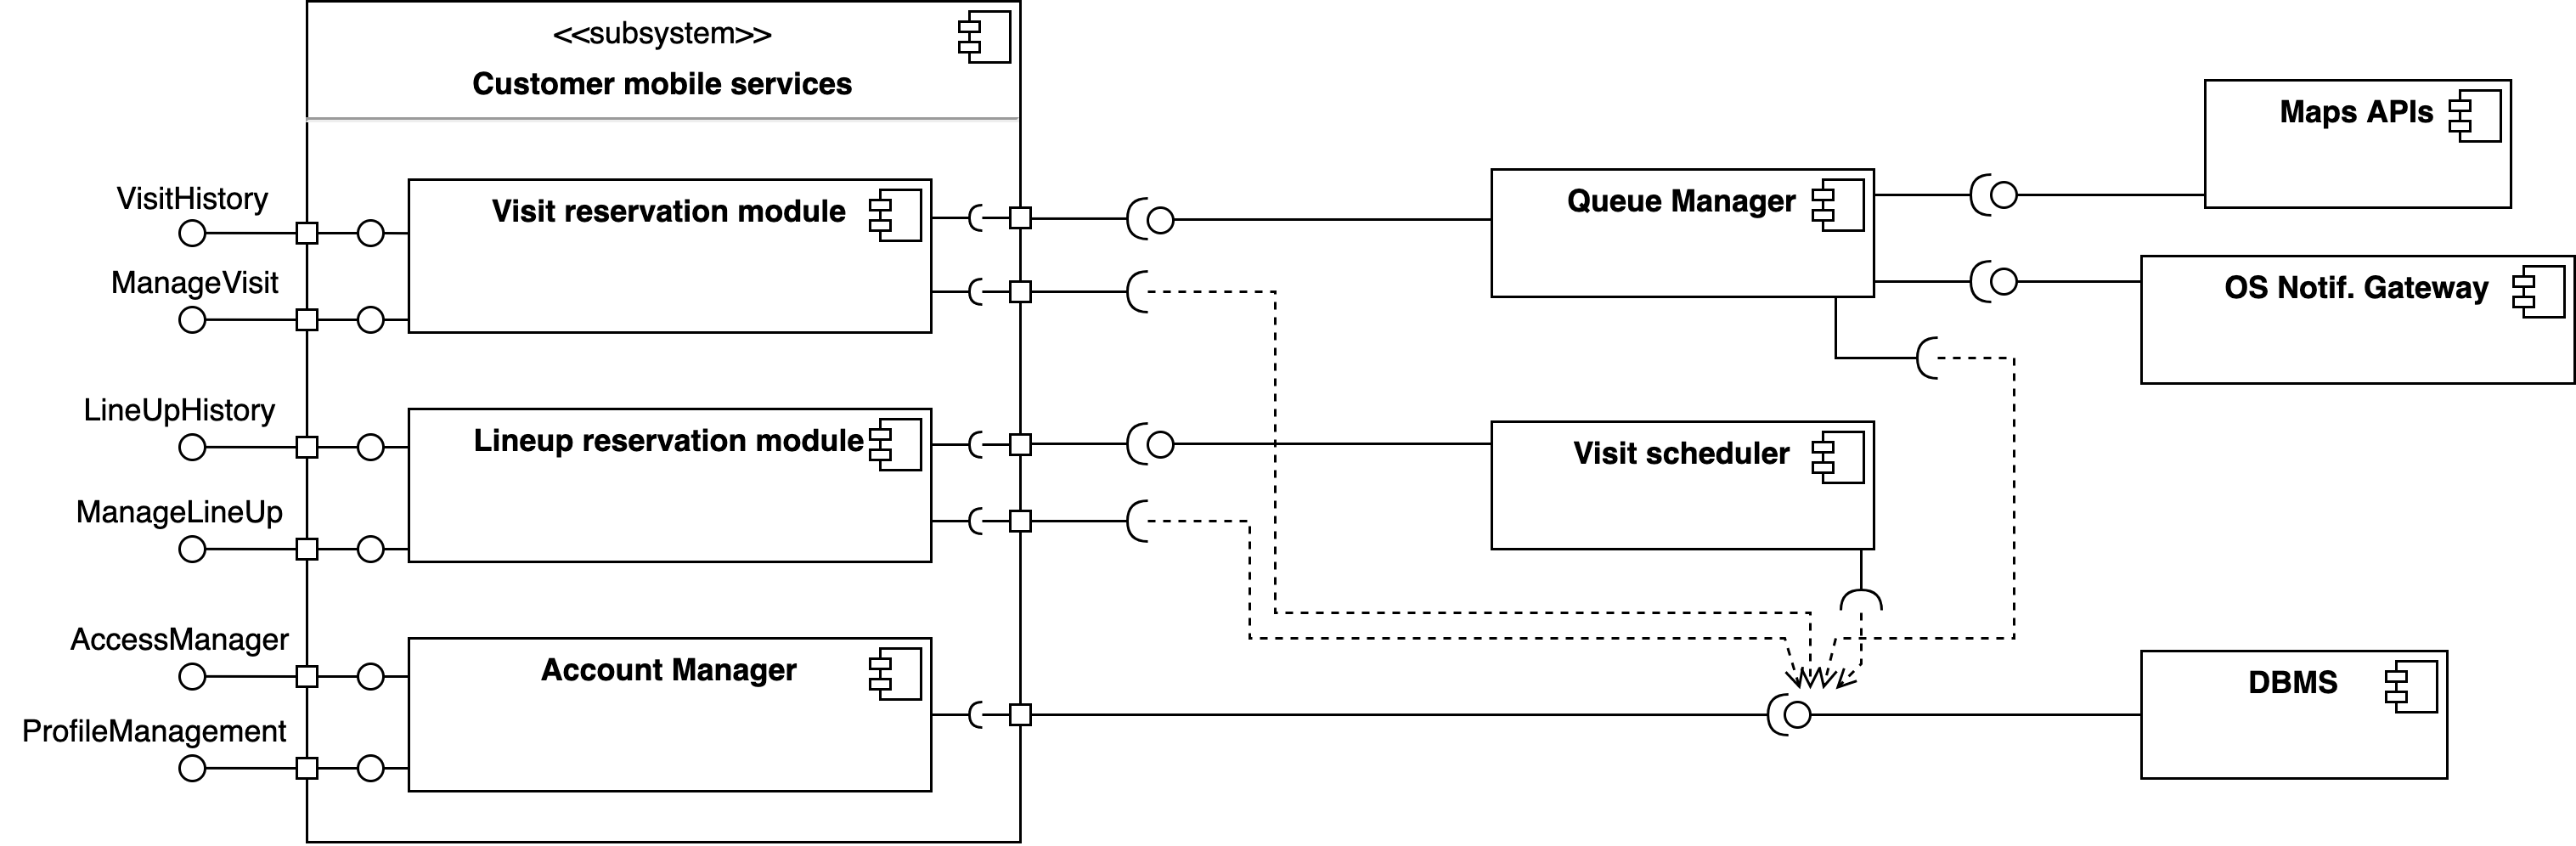
\includegraphics[width=16cm]{component_view-Customer_mobile_services.png}
        \caption{Customer Mobile Services component diagram}
    \end{figure}

\subsection{Employee web services diagram}

    The following diagram shows how the subsystem \textbf{Employee Web Services} is composed and how its modules communicate with external modules. This subsystem contains 3 modules: a \textit{Line up Reservation Module}, a \textit{Entrances and Exits Module} and an \textit{Account Manager}. This modules provides to Web Application the following interfaces: \textit{LineUp}, \textit{ManageEntrances}, \textit{ManageExits}, \textit{AccessManager}. The components of the Employee Web Services subsystem need to communicate with the DBMS and the Queue Manager and indirectly with OS Notification Gateway.

    \begin{figure}[H]
        \centering
        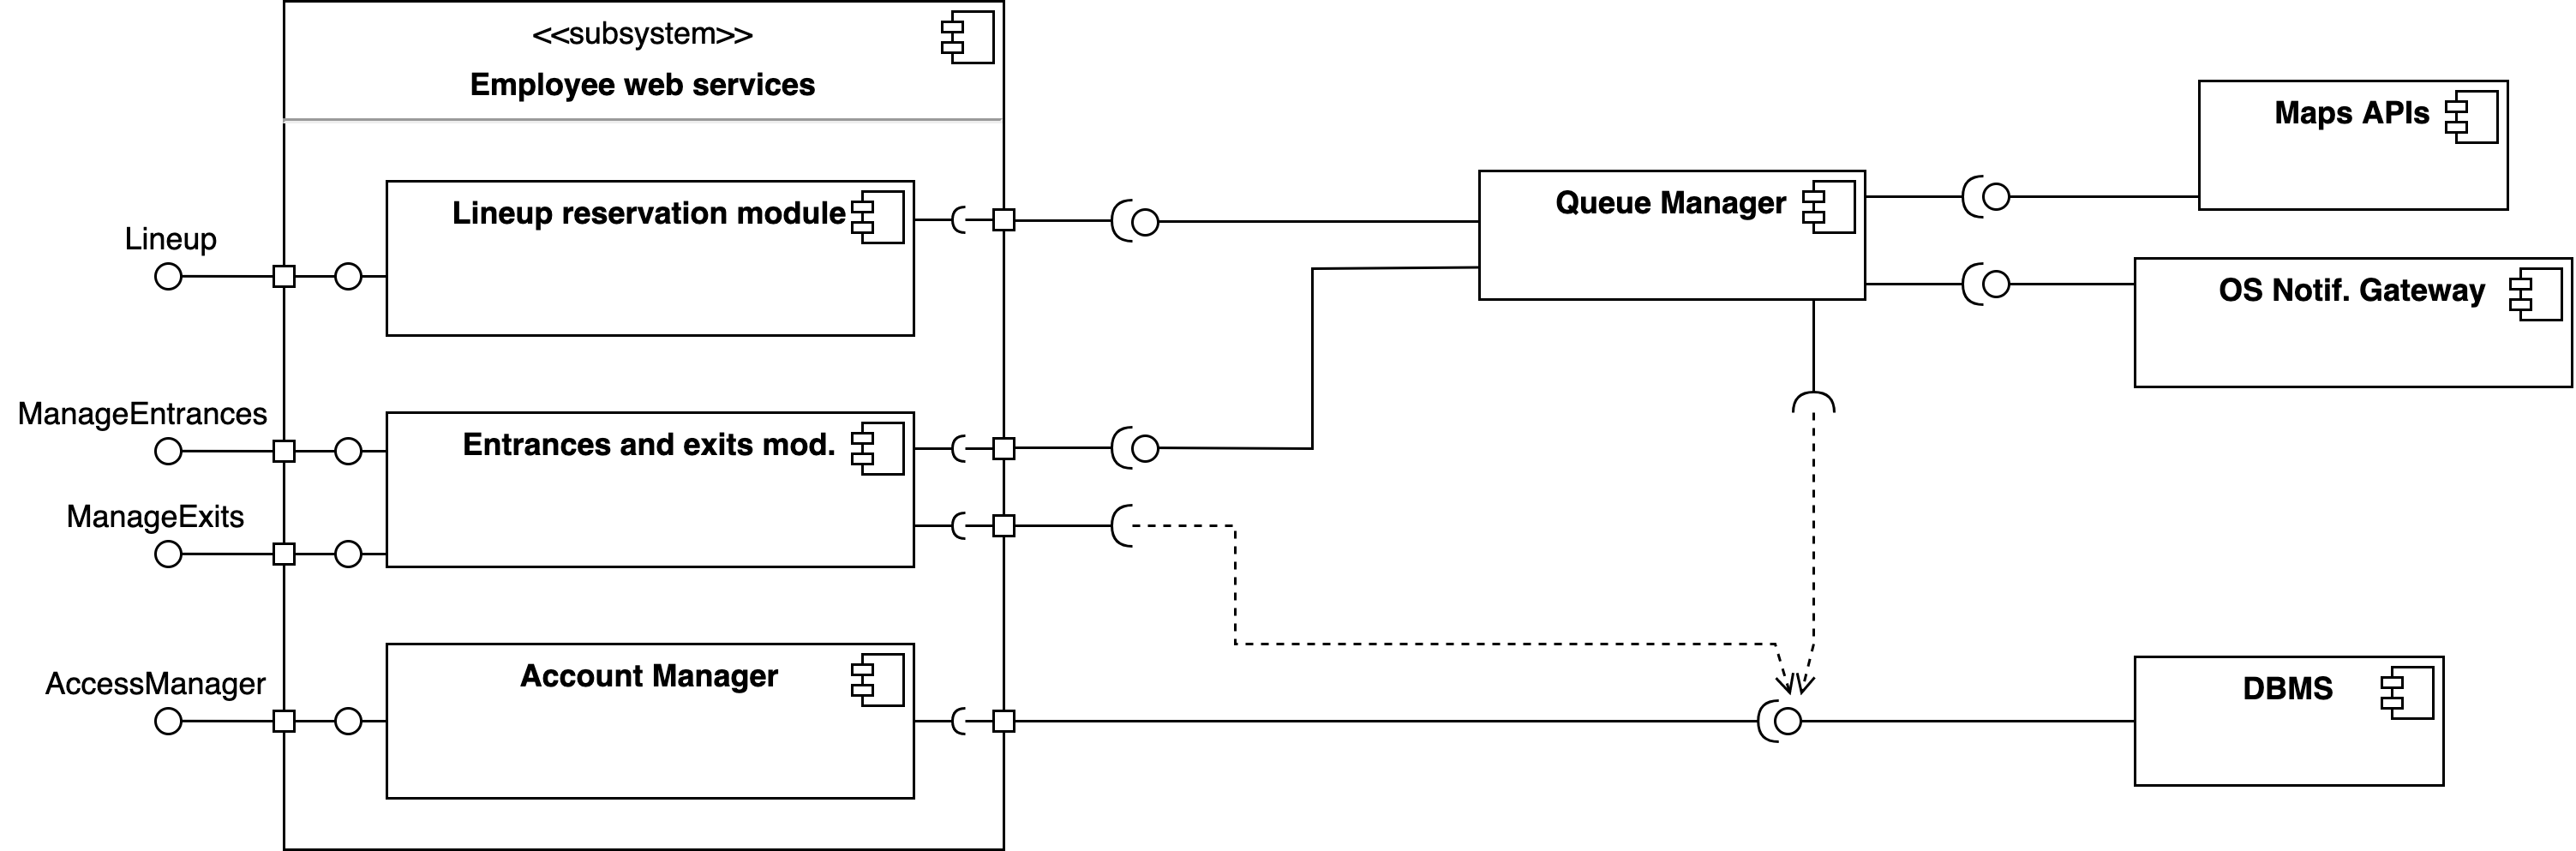
\includegraphics[width=16cm]{component_view-Employee_web_services.png}
        \caption{Employee Web Services component diagram}
    \end{figure}

\subsection{Store Manager web services diagram}

    The following diagram shows how the subsystem \textbf{Store Manager Web Services} is composed and how its modules communicate with external modules. This subsystem contains 3 modules: a \textit{Statistics and Data Gateway}, a \textit{Store Info and Employees Manager} and an \textit{Account Manager}. This modules provides to Web Application the following interfaces: \textit{Retrieve Statistics}, \textit{StoreManagement}, \textit{EmployeesManagement}, \textit{ProfileManagement}, \textit{AccessManager}. The components of the Store Manager Web Services subsystem need to communicate with the DBMS.

    \begin{figure}[H]
        \centering
        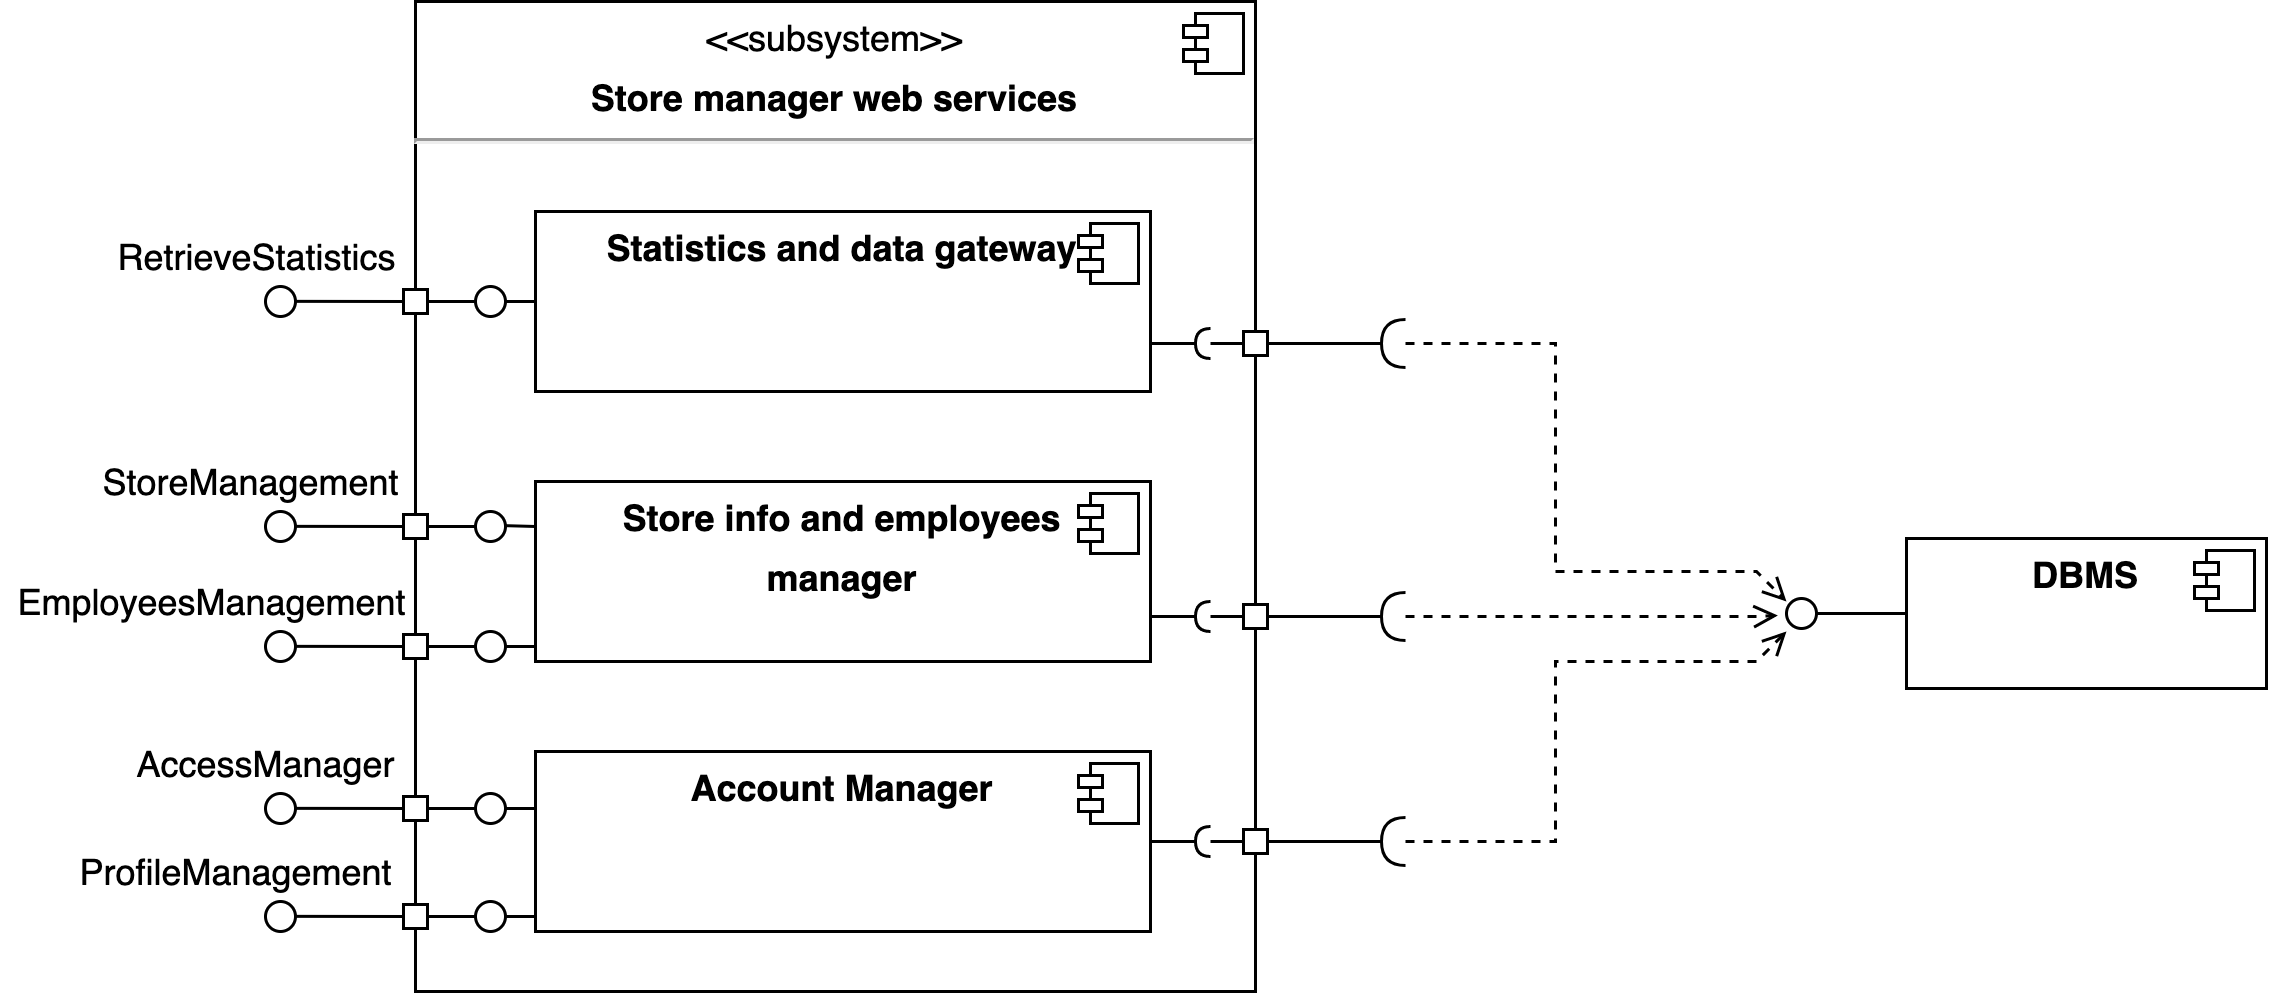
\includegraphics[width=16cm]{component_view-Store_manager_web_services.png}
        \caption{Store Manager Web Services component diagram}
    \end{figure}